\documentclass{article}

\usepackage{listings}
\usepackage{amsmath}
\usepackage{graphicx}
\usepackage{hyperref}
\usepackage{booktabs}
\usepackage{verbatim}
\usepackage{url}
\usepackage{framed}
\usepackage{booktabs}
\usepackage{mathtools}

\DeclarePairedDelimiter\abs{\lvert}{\rvert}%
\DeclarePairedDelimiter\norm{\lVert}{\rVert}%

\begin{document}

\title{Homework 12}
\author{Geoffrey Ulman\\
        CSI740}
\date{April 2012}
\maketitle

\section{Power Iteration}\label{p1}

The power iteration algorithm was implemented as specified in Algorithm 27.1 with the rate of change in the calculated eigenvalue used as a stopping condition. All calculations were run until the rate of change dropped below \(10^{-8}\).

Figures \ref{p1t1} and \ref{p1f1} summarize the convergence rate of the power iteration algorithm on the \(A\) matrix for a random initialization vector. Figure \ref{p1f1} plots the difference between the actual largest eigenvalue (as calculated by Matlab's \verb|eig| command) and the calculated eigenvalue on a log scale. Figure \ref{p1t1} prints these differences in tabular form. From these results we observe that each iteration improves the accuracy of the result by approximately three digits. This is a linear convergence rate (the error is decreasing by a constant multiple every iteration).

\begin{equation}
R_m=\abs*{\frac{\lambda_2}{\lambda_1}}^2
\label{eq2}
\end{equation}

Theorem 27.1 tells us to expect the error to decrease by the constant multiple \(R_m\) (given by equation \ref{eq2}) at every iteration. Figure \ref{p1f2} plots the \(R_m\) ratio at each iteration. The blue line indicates the square of the ratio between the true second-largest and largest eigenvalues of \(A\) as calculated by Matlab's \verb|eig| command. These values match quite well with the observed improvement of three digits of accuracy per step.

Finally, Figure \ref{p1f3} summarizes the number of iterations necessary to meet the stopping criteria for 1000 runs of the power iteration algorithm, each with a different random initial vector. A small number of initial vectors required one additional or one less iteration to converge. However, in general the choice of initial vector has little to no impact on the convergence rate. Of course, if a degenerate vector is chosen, like the zero vector or one of the other eigenvectors of \(A\), then the algorithm may fail.

\begin{figure}
\centering
\begin{tabular}{lrr}
\toprule
Iteration & Eigenvalue & Error \\
\midrule
 1 & 332.7815351291716 & 0.064780277883358 \\
 2 & 332.8461979585259 & 0.000117448529011 \\
 3 & 332.8463151514994 & 0.000000255555506 \\
 4 & 332.8463154064969 & 0.000000000558032 \\
 5 & 332.8463154070536 & 0.000000000001307 \\
 6 & 332.8463154070549 & 0.000000000000057 \\
\bottomrule
\label{p1t1}
\end{tabular}
\caption{Power Iteration: Error in Calculated Eigenvalue by Iteration}
\end{figure}

\begin{figure}
\centering
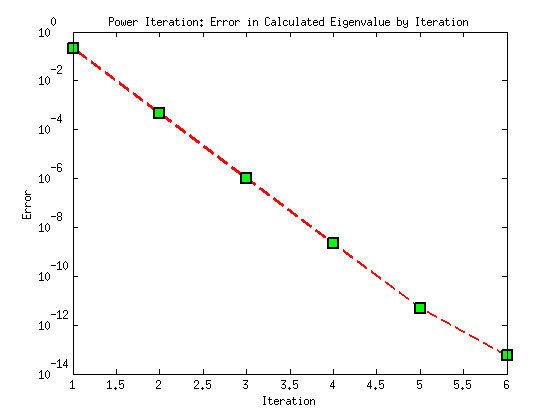
\includegraphics[width=0.8\textwidth]{Problem1Figure1.png}
\caption{Power Iteration: Error in Calculated Eigenvalue by Iteration}
\label{p1f1}
\end{figure}

\begin{figure}
\centering
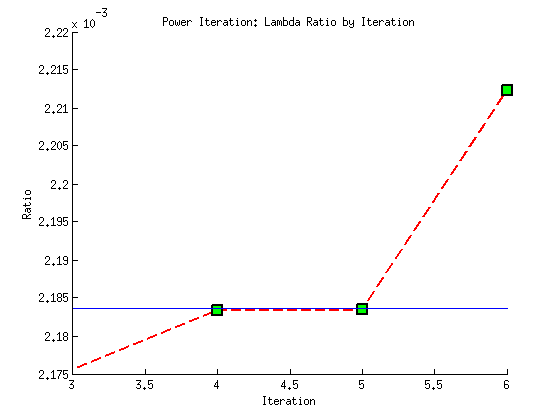
\includegraphics[width=0.8\textwidth]{Problem1Figure2.png}
\caption{Power Iteration: Lambda Ratio by Iteration}
\label{p1f2}
\end{figure}

\begin{figure}
\centering
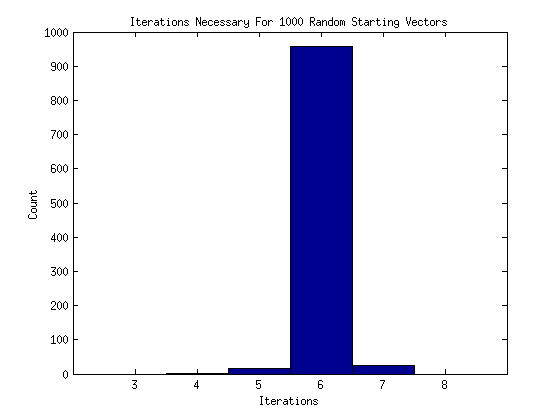
\includegraphics[width=0.8\textwidth]{Problem1Figure3.png}
\caption{Power Iteration: Iterations Necessary for 1000 Random Starting Vectors}
\label{p1f3}
\end{figure}

\section{Rayleigh Quotient Iteration}\label{p2}

Figures \ref{p2t1} and \ref{p2f1} summarize the convergence rate of the Rayleigh Quotient iteration algorithm on the \(A\) matrix for a random initialization vector. Figure \ref{p2f1} plots the difference between the actual largest eigenvalue (as calculated by Matlab's \verb|eig| command) and the calculated eigenvalue on a log scale. Figure \ref{p2t1} prints these differences in tabular form. The calculated eigenvalue converges much faster than for power iteration. There are no decimal places of accuracy on the first iteration, three on the second, and the calculated value exactly matches the value calculated by Matlab on the third iteration. This appears in line with the cubic convergence rate expected based on Theorem 27.3.

However, the choice of initial vector is significantly more important for the Rayleigh Quotient iteration algorithm. Whereas power iteration always converged to the largest eigenvalue in approximately the same number of iterations regardless of the choice of initial vector (barring a small number of degenerate choices), Rayleigh Quotient iteration can converge to any eigenvalue. Therefore, the chosen initial vector must be sufficiently close to the eigenvector corresponding to the eigenvalue we wish to find. Fortunately, it appears that the range of initial vectors which converge to the largest eigenvalues is significantly larger than for the smaller eigenvalues.

\begin{figure}
\centering
\begin{tabular}{lrr}
\toprule
Iteration & Eigenvalue & Error \\
\midrule
 1 & 329.4913308900763 & 3.354984516978561 \\
 2 & 332.8459395164913 & 0.000375890563589 \\
 3 & 332.8463154070549 & 0.000000000000000 \\
 4 & 332.8463154070549 & 0.000000000000000 \\
\bottomrule
\label{p2t1}
\end{tabular}
\caption{Rayleigh Quotient Iteration: Error in Calculated Eigenvalue by Iteration}
\end{figure}

\begin{figure}
\centering
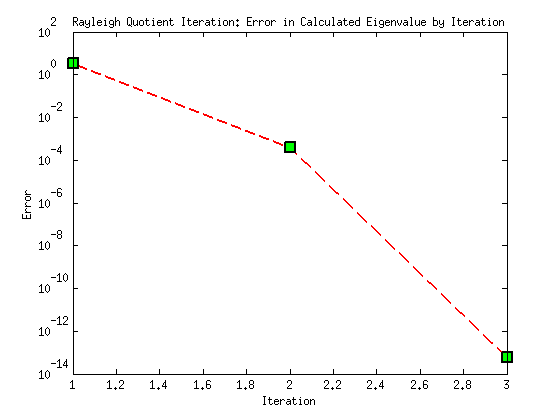
\includegraphics[width=0.8\textwidth]{Problem2Figure1.png}
\caption{Rayleigh Quotient Iteration: Error in Calculated Eigenvalue by Iteration}
\label{p2f1}
\end{figure}

\section{QR Iteration}\label{p3}

QR iteration was implemented according to Algorithm 28.1 with the magnitude of the largest off-diagonal lower-triangular element used as a stopping condition. All calculations were run until this value dropped below \(10^{-12}\).

Figure \ref{p3f1} charts the progression of this error over the 21 iterations necessary to reach the stopping condition. The final \(A\) matrix is shown by Figure \ref{p3m1}. Note that because \(A\) was symmetric, the QR iteration is converging to a diagonal matrix with the eigenvalues of \(A\) as the diagonal elements.

Figure \ref{p3f2} charts the same error metric for the non-symmetric \(A\) matrix. It is notable that the algorithm took significantly longer, 31 iterations instead of 21, to reach the stopping condition. The final \(A\) matrix is shown by Figure \ref{p3m2}. As expected, the matrix is upper-triangular instead of diagonal, but still contains the eigenvalues of \(A\) as diagonal elements.

\begin{figure}
\centering
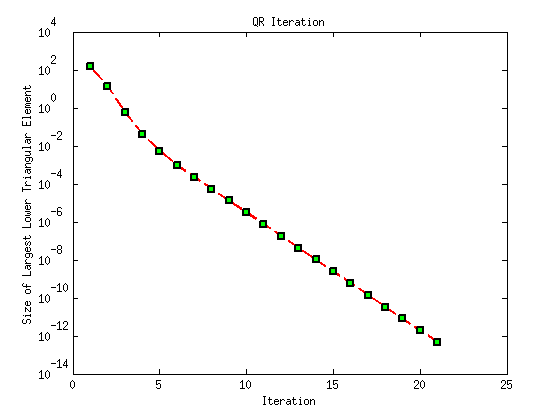
\includegraphics[width=0.8\textwidth]{Problem3Figure1.png}
\caption{QR Iteration: Magnitude of Largest Lower Triangular Element (Symmetric Input)}
\label{p3f1}
\end{figure}

\begin{figure}
\centering
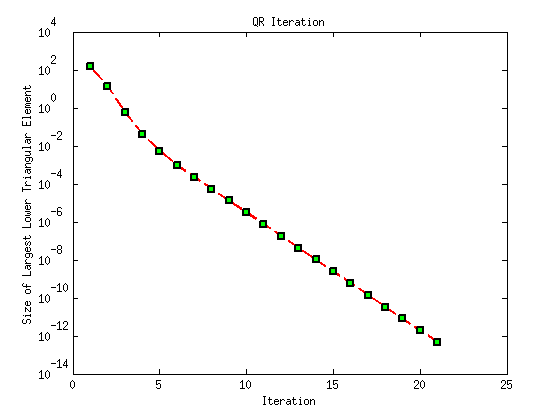
\includegraphics[width=0.8\textwidth]{Problem3Figure1.png}
\caption{QR Iteration: Magnitude of Largest Lower Triangular Element (Non-Symmetric Input)}
\label{p3f2}
\end{figure}

\begin{figure}
\centering
\(
\begin{bmatrix}
  332.8463 &  -0.0000 &  -0.0000 &   0.0000 &   0.0000 &  -0.0000 \\[0.3em]
    0.0000 &  15.5535 &  -0.0000 &   0.0000 &  -0.0000 &  -0.0000 \\[0.3em]
    0.0000 &   0.0000 &   2.0436 &   0.0000 &  -0.0000 &   0.0000 \\[0.3em]
    0.0000 &   0.0000 &   0.0000 &   0.4893 &   0.0000 &   0.0000 \\[0.3em]
    0.0000 &   0.0000 &   0.0000 &   0.0000 &   0.0643 &  -0.0000 \\[0.3em]
    0.0000 &   0.0000 &   0.0000 &   0.0000 &   0.0000 &   0.0030
\end{bmatrix}
\)
\label{p3m1}
\caption{QR Iteration End Result (Symmetric Input)}
\end{figure}


\begin{figure}
\centering
\(
\begin{bmatrix}
  332.8421 & -0.1042  & 0.3624 & -0.7312 &  0.2155 & -0.1595 \\[0.3em]
    0.0000 & 15.5913  & 0.2005 & -0.3372 &  0.1193 & -0.0774 \\[0.3em]
    0.0000 &  0.0000  & 1.9256 & -0.2344 & -0.0001 & -0.0377 \\[0.3em]
    0.0000 &  0.0000  & 0.0000 &  0.6019 &  0.1396 & -0.0270 \\[0.3em]
    0.0000 &  0.0000  & 0.0000 &  0.0000 &  0.0267 & -0.0225 \\[0.3em]
    0.0000 &  0.0000  & 0.0000 &  0.0000 &  0.0000 &  0.0125
\end{bmatrix}
\)
\label{p3m2}
\caption{QR Iteration End Result (Non-Symmetric Input)}
\end{figure}

\end{document}
